\documentclass[a4paper]{article}
\usepackage{cmap}  
\usepackage{vntex}
%\usepackage[english,vietnam]{babel}
%\usepackage[utf8]{inputenc}
%\usepackage[utf8]{inputenc}
%\usepackage[francais]{babel}
\usepackage{a4wide,amssymb,epsfig,latexsym,multicol,array,hhline,fancyhdr}

\usepackage{amsmath}
\usepackage{lastpage}
%\usepackage[lined,boxed,commentsnumbered]{algorithm2e}
\usepackage{enumerate}
\usepackage{color}
\usepackage{graphicx}							% Standard graphics package
\usepackage{array}
\usepackage{tabularx, caption}
\usepackage{multirow}
\usepackage{multicol}
\usepackage{rotating}
\usepackage{graphics}
\usepackage{geometry}
\usepackage{setspace}
\usepackage{epsfig}
\usepackage{tikz}
\usetikzlibrary{arrows,snakes,backgrounds}
\usepackage[unicode]{hyperref}
\hypersetup{urlcolor=blue,linkcolor=black,citecolor=black,colorlinks=true} 
%\usepackage{pstcol} 								% PSTricks with the standard color package


\usepackage{pifont}% http://ctan.org/pkg/pifont
\newcommand{\cmark}{\ding{51}}%
\newcommand{\xmark}{\ding{55}}%

%\usepackage{fancyhdr}
\setlength{\headheight}{40pt}
\pagestyle{fancy}
\fancyhead{} % clear all header fields
\fancyhead[L]{
 \begin{tabular}{rl}
    \begin{picture}(25,15)(0,0)
    \put(0,-8){
\includegraphics[width=8mm, height=8mm]{LogoBK.jpg}}
    %\put(0,-8){\epsfig{width=10mm,figure=hcmut.eps}}
   \end{picture}&
	\begin{tabular}{l}
		\textbf{\bf \ttfamily Faculty of Computer Science and Engineering}\\
		\textbf{\bf \ttfamily Bach Khoa University}
	\end{tabular} 	
 \end{tabular}
}
\fancyhead[R]{
	\begin{tabular}{l}
		\tiny \bf \\
		\tiny \bf 
	\end{tabular}  }
\fancyfoot{} % clear all footer fields
\fancyfoot[L]{\scriptsize \ttfamily Report Internet of Things  Application Development - Year 2017-2018}
\fancyfoot[R]{\scriptsize \ttfamily Page {\thepage}/\pageref{LastPage}}
\renewcommand{\headrulewidth}{0.3pt}
\renewcommand{\footrulewidth}{0.3pt}


%%%
%\setcounter{secnumdepth}{4}
%\setcounter{tocdepth}{3}
%\makeatletter
%\newcounter {subsubsubsection}[subsubsection]
%\renewcommand\thesubsubsubsection{\thesubsubsection .\@alph\c@subsubsubsection}
%\newcommand\subsubsubsection{\@startsection{subsubsubsection}{4}{\z@}%
%                                     {-3.25ex\@plus -1ex \@minus -.2ex}%
%                                     {1.5ex \@plus .2ex}%
%                                     {\normalfont\normalsize\bfseries}}
%\newcommand*\l@subsubsubsection{\@dottedtocline{3}{10.0em}{4.1em}}
%\newcommand*{\subsubsubsectionmark}[1]{}
%\makeatother



\begin{document}

\begin{titlepage}
\begin{center}
Faculty of Computer Science and Engineering\\
Ho Chi Minh City University of Technology
\end{center}

\vspace{.51cm}

\begin{figure}[h!]
\begin{center}

\includegraphics[width=3cm]{LogoBK.jpg}
\end{center}
\end{figure}

\vspace{0.5cm}


\begin{center}
\begin{tabular}{c}
\multicolumn{1}{l}{\textbf{{\Large \textcolor{blue}{PHÁT TRIỂN ỨNG DỤNG INTERNET OF THINGS}}}}\\
~~\\
\hline
\\
\multicolumn{1}{l}{\textbf{{\Large \textcolor{blue}{Đề Tài}}}}\\
\\
\textbf{{\Huge \textcolor{blue}{Hệ Thống An Ninh Với}}} \\
\textbf{{\Huge \textcolor{blue}{Raspberry Pi 3}}}\\
\\
\hline
\end{tabular}
\end{center}

\vspace{3cm}

\begin{table}[h]
\begin{tabular}{rrll}
\hspace{5 cm} & GV Hướng Dẫn: & Nguyễn Trần Hữu Nguyên&\\
& & Lê Trọng Nhân & \\
& Sinh viên: & Nguyễn Thành Đạt & 1510700 \\
& & Dương Vọng & 1514090 \\ 
& & Trần Quốc Khánh & 1511524\\ 
& & Huỳnh Thanh Duy& 1510450\\ 
\end{tabular}
\end{table}

\begin{center}
{\footnotesize Bach Khoa, 12/2018}
\end{center}
\end{titlepage}


%\thispagestyle{empty}
\newpage
\tableofcontents
\newpage

%%%%%%%%%%%%%%%%%%%%%%%%%%%%%%%%%
\section{Mô tả đề tài}
\hspace{6mm} Sản phẩm nhóm cung cấp sẽ là hệ thống nhận cho phép xác định đối tượng các tòa nhà, công sở,.... Các trạm ra vào tòa nhà, cũng như các cửa phòng ban sẽ được gắn một đầu đọc thẻ từ RCC và camera tùy vào ưu tiên của vị trí đó. Nhân viên cũng như người sử dụng muốn qua hệ thống an ninh phải đủ quyền hạn ở cống đó. Ngoài ra còn các vị trí tùy vào mức độ ưu tiên sẽ được gắn camera và theo dõi trực tiếp trên trang quản lý hệ thống. Server có thể phát hiện ra danh tính của nhân viên dựa trên hình ảnh thu thập được.
\section{Chức năng}
	Một số chức năng:
	\begin{itemize}
		\item Quét thẻ xác định quyền mở cửa.  
		\item Có nhiều phòng ban, mỗi phòng ban có nhiều cửa, mỗi cửa có một cấp độ riêng, chỉ những người sở hữu loại thẻ có cùng hoặc cấp độ cao hơn mới có quyền mở cửa.
		\item Thêm, xóa, cấp quyền cho nhân viên.
		\item Thêm, xóa, xác định yêu cầu mở cửa cho cửa.
		\item Thêm, xóa phòng ban và thiết lập quyền.
		\item Hệ thống ghi lại nhật ký mở cửa bao gồm tên nhân viên, tên cửa, phòng ban và hình ảnh của nhân viên mở cửa.
	\end{itemize}
\section{Công cụ sử dụng}
\subsection{Đầu đọc RCC}
\subsection{Thẻ từ}
\hspace{6mm} Là loại là thẻ dùng từ tính để tích hợp với đầu đọc thẻ hoặc máy chấm công cảm ứng. Thường được sử dụng như thẻ ID, thẻ nhân viên, thẻ chấm công, thẻ chìa khóa…rất tiện lợi cho việc chấm công ra vào, tiết kiệm thời gian.
\subsection{Hệ cơ sở dữ liệu MongoDb}
\hspace{6mm} Sử dụng hệ cơ sở dữ liệu MongoDb để lưu và truy vấn dữ liệu. Cở sở dữ liệu gồm có:
\\
\begin{figure}[h!]
\begin{center}
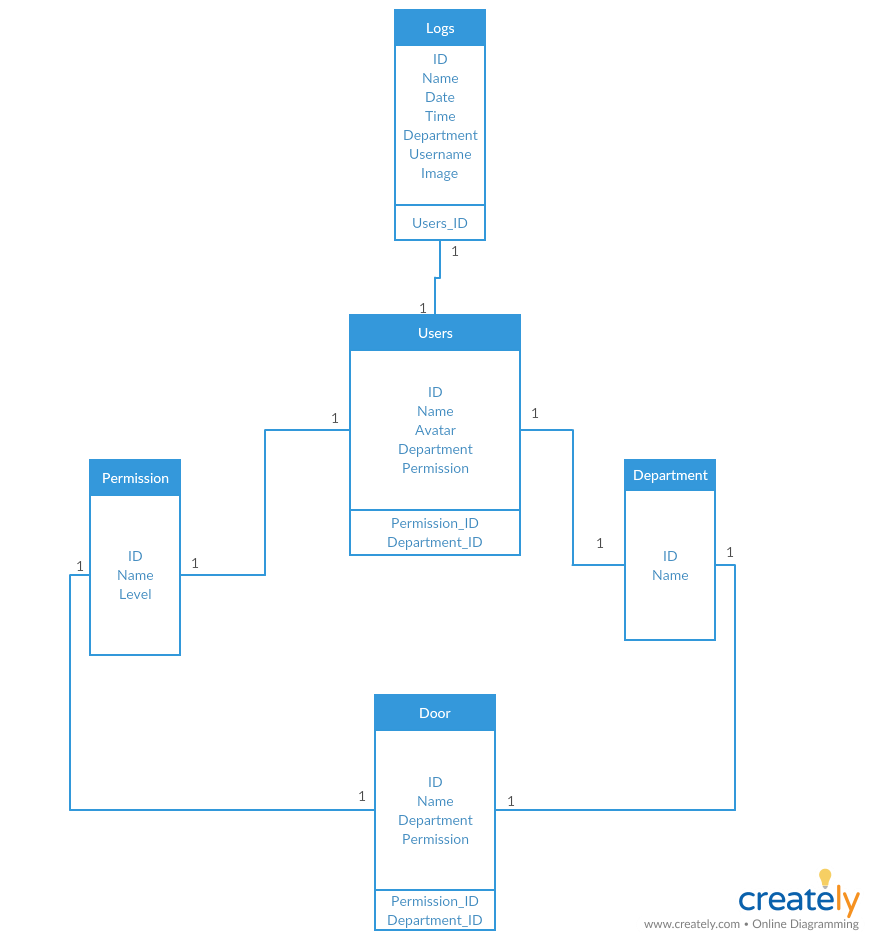
\includegraphics[width=11cm]{db_diagram.png}
\\Lược đồ database
\end{center}
\end{figure}
\subsection{Nodejs}
\hspace{6mm} Nodejs là một nền tảng (Platform) phát triển độc lập được xây dựng ở trên Javascript Runtime của Chrome mà chúng ta có thể xây dựng được các ứng dụng mạng một cách nhanh chóng và dễ dàng mở rộng. Tạo ra được các ứng dụng có thể xử lý nhanh, realtime.
Nhóm sử dụng nodejs để viết server, công nghệ Socket io để giao tiếp với Raspberry. 


\section{Quá trình thử nghiệm}
\subsection{Hướng dẫn sử dụng}
\hspace{6mm}
\begin{itemize}
    \item Tại thư mục Face-Recognition-ON-Rasp mở terminal chạy lệnh "npm install" để cài các module cần thiết.
    \item Chạy lệnh "npm start" để khởi động server (nhóm sử dụng package nodemon để server tự cập nhập khi có sửa đổi). Truy cập vào địa chỉ http:\\localhost:3000.
    \item Nhập user name và password là "admin" để truy cập vào hệ thống.
    \item Truy cập trang User để nhận được trang List User click vào button add new User để thêm User. tương tự ới các trang Door, Department, Permission.
    \item Truy cập trang Log để xem nhật ký.
    \item Dùng thẻ quét qua Raspberry, Raspberry sau khi nhận được id người dùng từ thẻ, sẽ lấy được permission của người dùng từ database, đối chiếu với permission đã được thiết lập trên Rasp và xác định mở hoặc đóng cửa.
\end{itemize}


\subsection{Kết quả}
\hspace{6mm} Nhóm kiểm tra và hệ thống chạy khá ổn định.
\begin{figure}[h!]
\begin{center}
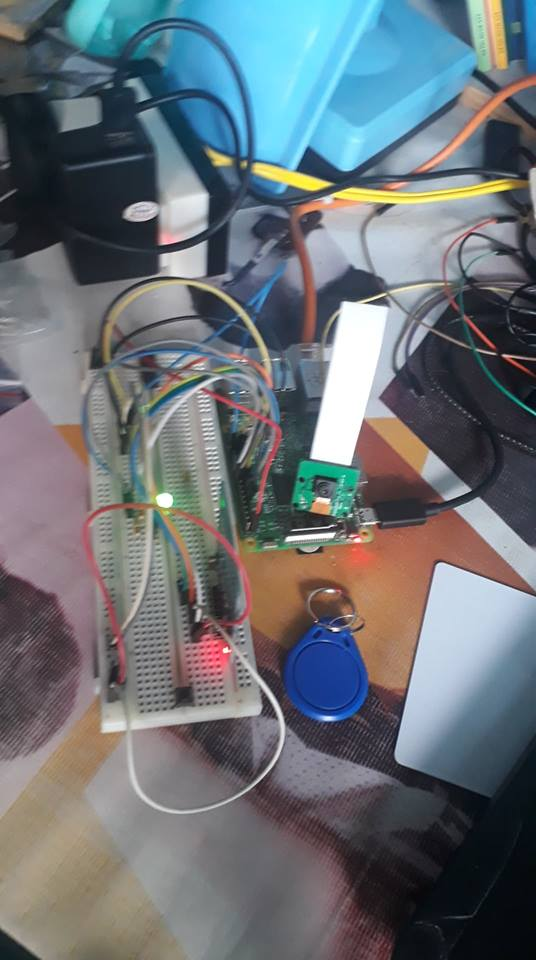
\includegraphics[width=9cm]{rasp_board.jpg}
\\Board mạch
\end{center}
\end{figure}
\section{Hướng phát triển}
Dự án có thể phát triển lên thành sản phẩm dùng trong các hộ gia đình lẫn công ty, cơ quan, nơi công cộng. Các tính năng sẽ được nâng cấp về sau.

\section{Kết luận}
Đây là sản phẩm hiệu quả, góp phần vào cuộc cách mạng 4.0 của Việt Nam.

\section{Tham khảo}
Link source code + report: \url{https://github.com/ad0min/Android-Thing-Raspberry-Pi-3B/tree/master/Face-Recognition-On-Rasp}
%%%%%%%%%%%%%%%%%%%%%%%%
%%%%%%%%%%%%%%%%%%%%%%%%%%%%%%%%%


 
\end{document}

